%\documentclass[tikz, border=5pt]{standalone}
\begin{document}
	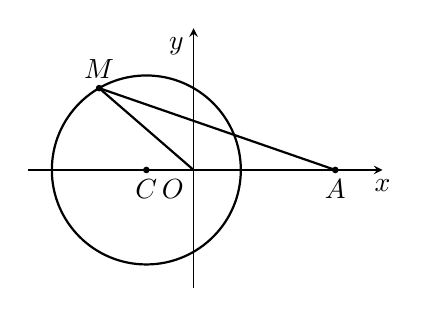
\begin{tikzpicture}[>=stealth, scale=0.6]
		% 绘制坐标轴
		\draw[->] (-3.5,0) -- (4,0) node[below ] {$x$};
		\draw[->] (0,-2.5) -- (0,3) node[below left] {$y$};
		\node at (0,0) [below left] {$O$};
		
		% 绘制圆(圆心在原点,半径设为2)
		\draw[thick] (-1,0) circle (2);
		
		% 定义切点M的坐标(M(√2, √2),在圆上且位于第一象限)
		\coordinate (A) at (3,0);
		\coordinate (C) at (-1,0);
		\coordinate (M) at (-2,{sqrt(3)});
		
		% 绘制从原点到切点M的线段(虚线)
		\draw[thick] (0,0) -- (M);
		\draw[thick] (A) -- (M);
		
		% 标记切点M
		\fill (M) circle (2pt) node[above ] {$M$}; % 圆上的点
		\fill(A) circle (2pt) node (A) [below] {$A$};
		\fill(C) circle (2pt) node (C) [below] {$C$};
		
	\end{tikzpicture}
\end{document}
